\documentclass{article}
\usepackage{tikz}
\usetikzlibrary{arrows.meta}

\begin{document}

\begin{figure}[h]
    \centering
    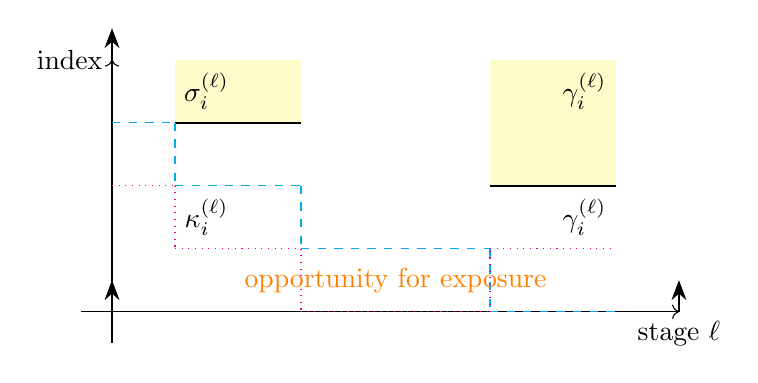
\begin{tikzpicture}[scale=0.8]
        % Axes
        \draw[->] (-0.5,0) -- (9,0) node[below] {stage $\ell$};
        \draw[->] (0,-0.5) -- (0,4) node[left] {index};

        % Boxes
        \fill[yellow!20] (1,3) rectangle (3,4);
        \fill[yellow!20] (6,2) rectangle (8,4);

        % Lines
        \draw[thick, black] (1,3) -- (3,3);
        \draw[thick, black] (6,2) -- (8,2);

        % Dashed lines
        \draw[dashed, cyan] (0,3) -- (1,3);
        \draw[dashed, cyan] (1,3) -- (1,2);
        \draw[dashed, cyan] (1,2) -- (3,2);
        \draw[dashed, cyan] (3,2) -- (3,1);
        \draw[dashed, cyan] (3,1) -- (6,1);
        \draw[dashed, cyan] (6,1) -- (6,0);
        \draw[dashed, cyan] (6,0) -- (8,0);

        % Dotted lines
        \draw[dotted, magenta] (0,2) -- (1,2);
        \draw[dotted, magenta] (1,2) -- (1,1);
        \draw[dotted, magenta] (1,1) -- (3,1);
        \draw[dotted, magenta] (3,1) -- (3,0);
        \draw[dotted, magenta] (3,0) -- (6,0);
        \draw[dotted, magenta] (6,0) -- (6,1);
        \draw[dotted, magenta] (6,1) -- (8,1);

        % Labels
        \node at (1.5,3.5) {$\sigma_i^{(\ell)}$};
        \node at (7.5,3.5) {$\gamma_i^{(\ell)}$};
        \node at (1.5,1.5) {$\kappa_i^{(\ell)}$};
        \node at (7.5,1.5) {$\gamma_i^{(\ell)}$};
        \node at (4.5,0.5) {\textcolor{orange}{opportunity for exposure}};

        % Arrows
        \draw[-{Stealth[scale=1.5]}] (0,0) -- (0,0.5);
        \draw[-{Stealth[scale=1.5]}] (9,0) -- (9,0.5);
        \draw[-{Stealth[scale=1.5]}] (0,4) -- (0,4.5);
    \end{tikzpicture}
    \caption{One realization of the Weitzman indices $\sigma_i^{(1)},\dots$ when opening nested boxes in a Pandora basket $i$. The minimum index so far is $\gamma_i^{(\ell)}$ and the minimum yet to come (including the final value) is the capped value $\kappa_i^{(\ell)}$. Yellow regions represent possible opportunities for exposure: if the index $\sigma_i^{(\ell)}$ of the next box under consideration is higher than the current $\gamma_i^{(\ell-1)}$, it is possible that $\kappa_i^{(\ell)}> \gamma_i^{(\ell - 1)}$, in which case failing to continue opening would cause exposure.}
\end{figure}

\end{document}